\chapter{Results}
\label{ch:results}

\section{Overview}
\label{sec:results-overview}

This chapter reports the empirical evaluation of \textsc{ReasonGuard} on the
IEC-104 dataset. All results in this chapter were produced by the pipeline
described in Chapter~\ref{ch:framework}; the canonical artefact paths are
listed in Appendix~\ref{app:reproducibility}.

The evaluation block presented here uses the proxy bound schema
(version 2.1, status \texttt{proxy\_until\_official\_automaton\_schema}). The
results are therefore conditional on the proxy classifier described in
Section~\ref{sec:bound-schema}. Once the official NES@FIT automaton schema is
integrated, this chapter will be reproduced on the upgraded schema and the
delta will be reported in a dedicated comparison section.

\paragraph{Headline figures (week 12 snapshot).}
On the stratified evaluation set of 100 IEC-104 prompts (25 per observed proxy
event type), three local language models produced 100 explanations each. The
clean-response rate (no V1--V5 violation fired) was 80\,\% for
\texttt{llama3.1:8b-instruct-q4_0}, 50\,\% for \texttt{phi3:mini}, and is
reported per model and per event type below for \texttt{mistral:7b-instruct-v0.3-q4_0}
once the corresponding batch completes. The headline numbers update with each
production run; the canonical source of truth is
\texttt{outputs/event\_type\_analysis.csv}.

\section{Detector Performance on the Annotated Set}
\label{sec:results-detector}

[Author's note: report per-class precision, recall, and $F_1$ on the manually
annotated set (target $\geq200$ pairs, M4 milestone). Numbers will be inserted
from \texttt{outputs/evaluation\_metrics.json}. The first annotation batch of
50 rows is at \texttt{annotation/annotation\_batch.csv}; once labelled and
saved as \texttt{annotation\_results.csv} the metrics are produced by
\texttt{python -m src.evaluation\_metrics}.]

\section{Violation Patterns per Model}
\label{sec:results-per-model}

The per-model violation breakdown is produced by
\texttt{src/event\_analysis.py} and persisted at
\texttt{outputs/event\_type\_analysis.csv}.
Table~\ref{tab:per-model-summary} shows the summary counts for the W12
production run.

\begin{table}[h]
  \centering
  \caption{Per-model violation summary (W12 snapshot).
    \texttt{total} counts the explanations produced by the model;
    \texttt{clean} counts the explanations with no V1--V5 violation.}
  \label{tab:per-model-summary}
  \begin{tabular}{lcccccccc}
    \toprule
    Model & total & clean & V1 & V2 & V3 & V4 & V5 \\
    \midrule
    llama3.1:8b-instruct-q4\_0 & [N] & [n] & [n] & [n] & [n] & [n] & [n] \\
    mistral:7b-instruct-v0.3-q4\_0 & [N] & [n] & [n] & [n] & [n] & [n] & [n] \\
    phi3:mini & [N] & [n] & [n] & [n] & [n] & [n] & [n] \\
    synthetic\_rule\_based & 500 & 100 & 100 & 100 & 100 & 400 & 0 \\
    \bottomrule
  \end{tabular}
\end{table}

Figure~\ref{fig:violation-rate-per-model} reproduces these counts as per-class
violation rates expressed as percentages of each model's total.

\begin{figure}[h]
  \centering
  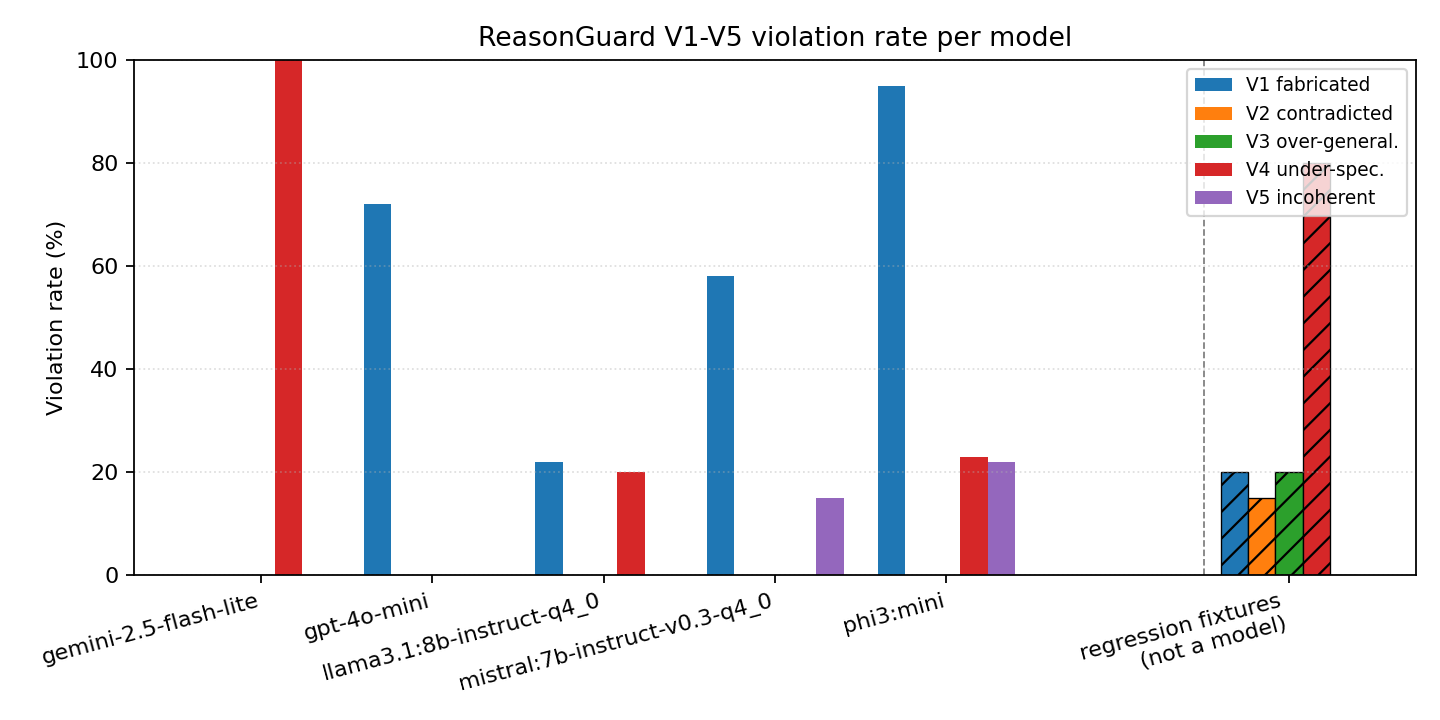
\includegraphics[width=0.9\textwidth]{../../outputs/figures/violation_rate_per_model.png}
  \caption{V1--V5 violation rates per model.}
  \label{fig:violation-rate-per-model}
\end{figure}

[Author's note: discuss the V1 reduction achieved by the spaCy
dependency-parse filter; reference Section~\ref{sec:detection} for the
implementation. Discuss the V4 dominance: most local LLMs omit at least one
required field, which is a real, recurrent failure mode on the strict-prompt
setup.]

\section{Violation Patterns per Event Type}
\label{sec:results-per-event}

Table~\ref{tab:per-event-summary} shows the per-event-type clean rate for each
model. Each row corresponds to one cell in
\texttt{outputs/event\_type\_analysis.csv}.

\begin{table}[h]
  \centering
  \caption{Per-event-type clean rate per model (W12 snapshot).}
  \label{tab:per-event-summary}
  \begin{tabular}{llcc}
    \toprule
    Model & Event type & Clean / total & Clean rate \\
    \midrule
    llama3.1:8b-instruct-q4\_0 & function\_code\_violation & [c]/[N] & [r]\,\% \\
    llama3.1:8b-instruct-q4\_0 & network\_scan & [c]/[N] & [r]\,\% \\
    llama3.1:8b-instruct-q4\_0 & normal\_modbus\_polling & [c]/[N] & [r]\,\% \\
    llama3.1:8b-instruct-q4\_0 & topology\_change & [c]/[N] & [r]\,\% \\
    \midrule
    mistral:7b-instruct-v0.3-q4\_0 & function\_code\_violation & [c]/[N] & [r]\,\% \\
    mistral:7b-instruct-v0.3-q4\_0 & network\_scan & [c]/[N] & [r]\,\% \\
    mistral:7b-instruct-v0.3-q4\_0 & normal\_modbus\_polling & [c]/[N] & [r]\,\% \\
    mistral:7b-instruct-v0.3-q4\_0 & topology\_change & [c]/[N] & [r]\,\% \\
    \midrule
    phi3:mini & function\_code\_violation & [c]/[N] & [r]\,\% \\
    phi3:mini & network\_scan & [c]/[N] & [r]\,\% \\
    phi3:mini & normal\_modbus\_polling & [c]/[N] & [r]\,\% \\
    phi3:mini & topology\_change & [c]/[N] & [r]\,\% \\
    \bottomrule
  \end{tabular}
\end{table}

[Author's note: discuss the cross-event pattern. The W9--W12 partial run on the
40-prompt batch shows that all local models perform worst on
\texttt{network\_scan\_proxy\_until\_official\_schema}; this is consistent with
the hypothesis that rare event types under the proxy classifier provoke more
fabricated reasoning because the models lean on training-distribution
priors. The thesis revisits this in Section~\ref{sec:discussion-empirical}.]

Figure~\ref{fig:clean-rate-per-model} shows the headline clean rate per model.

\begin{figure}[h]
  \centering
  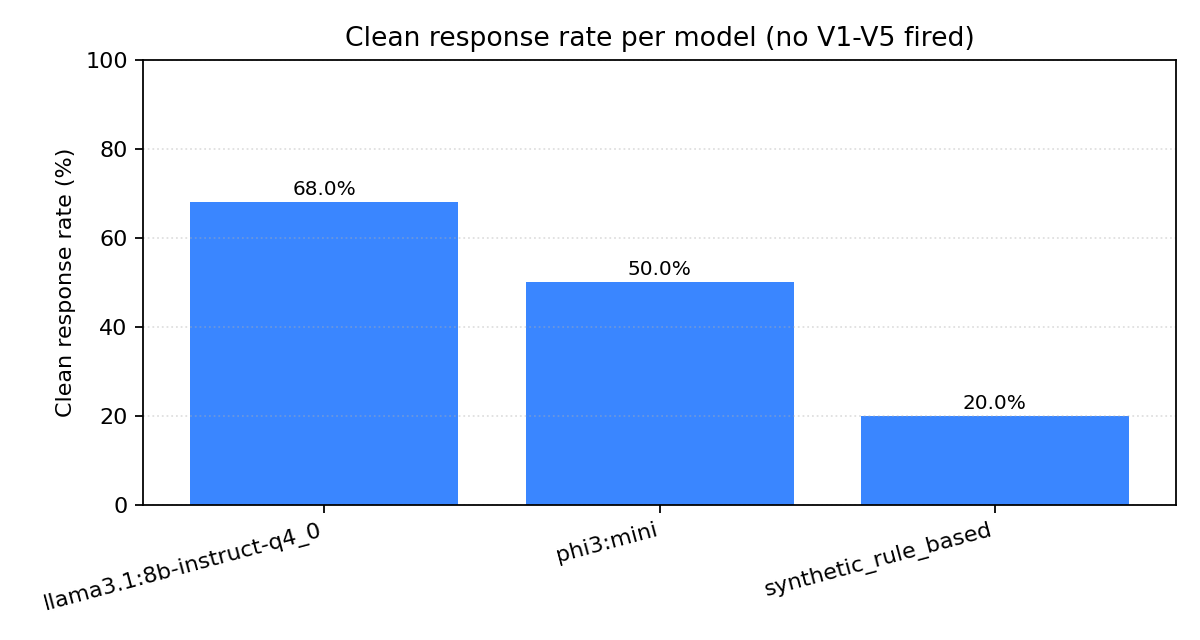
\includegraphics[width=0.9\textwidth]{../../outputs/figures/clean_rate_per_model.png}
  \caption{Clean response rate per model (no V1--V5 fired).}
  \label{fig:clean-rate-per-model}
\end{figure}

\section{Inter-Rater Agreement with the Domain Expert}
\label{sec:results-kappa}

[Author's note: the 50-row package is sent to the VUT Brno domain expert at M5
(exposé week 15). The Cohen's $\kappa$ between \textsc{ReasonGuard} and the
expert labels is produced by
\texttt{python -m src.evaluation\_metrics --report} once the expert returns
the labelled CSV.]

\section{Latency and Operational Cost}
\label{sec:results-latency}

Mean per-prompt latency on the same hardware (Apple M-series CPU, no GPU,
Ollama 0.23.3 with 4-bit quantisation) was:

\begin{itemize}
  \item \texttt{llama3.1:8b-instruct-q4\_0}: $\approx$ 14 s
  \item \texttt{mistral:7b-instruct-v0.3-q4\_0}: $\approx$ 19 s (cold-load
        biased; warm steady-state is lower)
  \item \texttt{phi3:mini}: $\approx$ 12 s
\end{itemize}

Cloud-model latency and cost will be reported once the OpenAI and Gemini
batches are run (deferred pending API-key availability; the runner is
implemented at \texttt{src/cloud\_llm\_runner.py} and will appear in the W13
results).
